\documentclass{beamer}

 \usepackage[francais]{babel}


\usepackage{tikz}
\usepackage[compat=1.1.0]{tikz-feynman}
\usetikzlibrary{angles, quotes}
\usetikzlibrary{calc}
\usetikzlibrary{decorations.pathreplacing, shapes.misc, arrows.meta}
\usepackage{pgfplots}


\usepackage[T1]{fontenc}
\UseRawInputEncoding
\usetheme{Warsaw}
\usepackage{pgfpages}
\usepackage{latexsym,xcolor,multicol,booktabs,calligra}
\usepackage{listings,stackengine}
\usepackage{subcaption}
\usepackage{tabularx}

\usepackage{QUT}

\usepackage{amsmath}
\usepackage{amssymb}
\usepackage{amsfonts}
\usepackage{mathtools}
\usepackage{physics}
\usepackage{graphicx}
\usepackage{dsfont}
\usepackage{xspace}

\definecolor{deepblue}{rgb}{0,0,0.5}
\definecolor{deepred}{rgb}{0.6,0,0}
\definecolor{deepgreen}{rgb}{0,0.5,0}
\definecolor{halfgray}{gray}{0.55}

\lstset{
    basicstyle=\ttfamily\small,
    keywordstyle=\bfseries\color{deepblue},
    emphstyle=\ttfamily\color{deepred},
    stringstyle=\color{deepgreen},
    numbers=left,
    numberstyle=\small\color{halfgray},
    rulesepcolor=\color{red!20!green!20!blue!20},
    frame=shadowbox,
}

\newcommand{\lemaitre}{\textsc{Lemaître}\xspace}
\newcommand{\credits}[1]{\tiny Credits : #1}


\title[Mesure de la croissance des structures avec DESI et ZTF]{Mesure de la croissance des structures avec les galaxies du DESI BGS et les supernovae de type Ia de ZTF : vers une analyse jointe}
\subtitle{Stage de fin d'études}
\author[Antoine Gilles--Lordet]{Antoine Gilles--Lordet \\ \footnotesize encadré par Pauline Zarrouk et Nicolas Regnault}
\date{10 octobre 2024}

\begin{document}

\frame{\titlepage}

\begin{frame}
	\tableofcontents
\end{frame}

\section{Introduction}

\subsection{Contexte}

%% 3 slides sur Lambda CDM, Energie noire, SNe Ia. Croissance des structures = derniers gros secteur à explorer

\begin{frame}{Cosmologie}
	Le modèle cosmologique actuel est $\Lambda$CDM, description remarquable
	Deux composantes, matière noire et énergie noire

	Domaine en plein essor : 3 projets à 1M\$ : Euclid, DESI, LSST... 	
\end{frame}

\begin{frame}{Matière noire et galaxies}
	Matière noire -> vitesses de rotation des galaxies et distribution de matière, structures.
	\begin{figure}
		\centering
		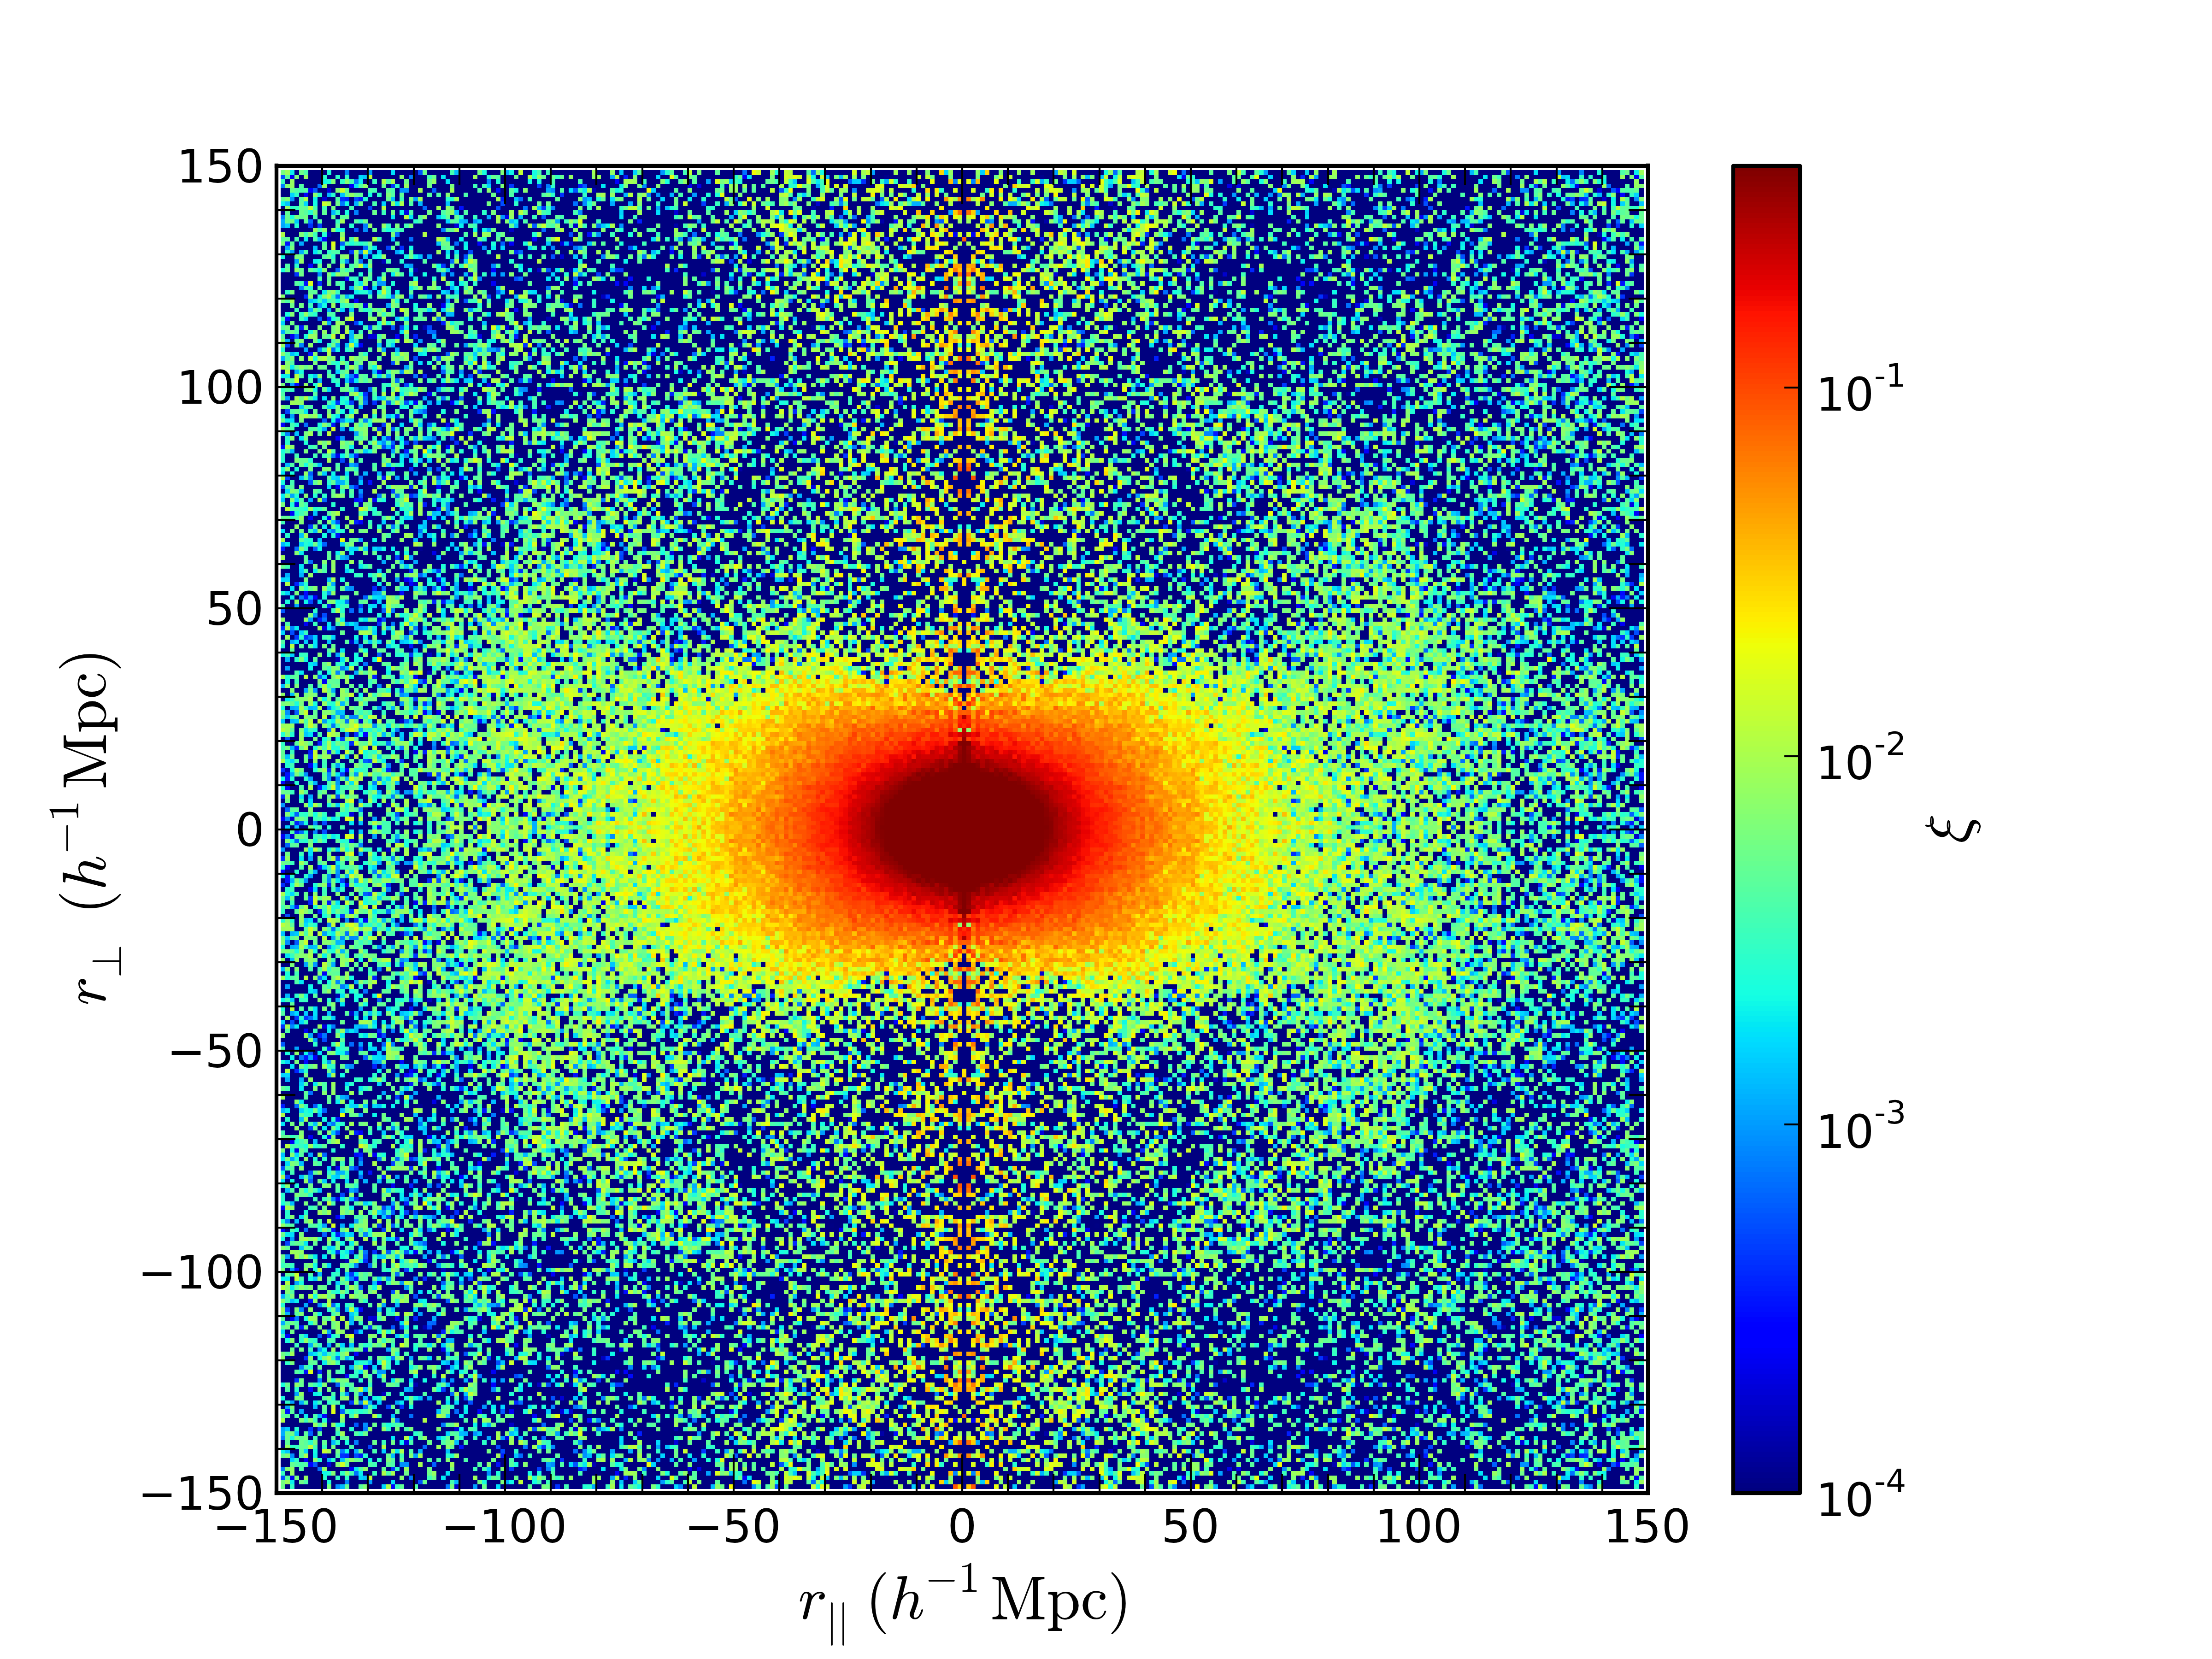
\includegraphics[height=0.5\textheight]{figures/FoG.png}
		\caption{Fonction de corrélation 2D des galaxies du relevé DR11 CMASS\\ \credits{SDSS Collaboration, Samushia et al. (2013)}}
	\end{figure}
\end{frame}

\begin{frame}{Energie noire et SNe Ia}
	La découverte de l'accélération de l'expansion de l'univers a été réalisée avec des SNeIa par S. Perlmutter, B. Schmidt et A. Riess
	\begin{figure}
		\centering
		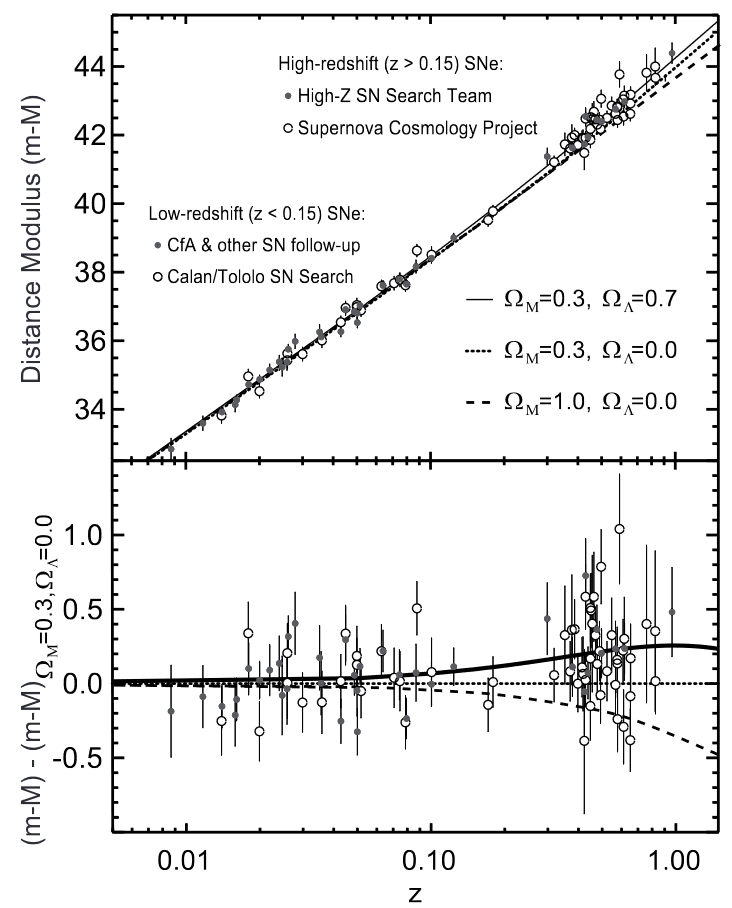
\includegraphics[height=0.5\textheight]{figures/Perlmutter_Schmidt.png}
		\caption{Diagramme de Hubble construit par Perlmutter et Schmidt en 2003}
	\end{figure}
\end{frame}

% Photo Telescopes
\subsection{ZTF}
\begin{frame}{ZTF}
\begin{columns}
\begin{column}{.5\textwidth}
	\begin{itemize}
		\item Situé à l'Observatoire de Palomar, utilise le telescope P48
		\item 1,22m de diamètre pour un champ de 47 degrés carré
		\item 16 CCDs de $6144 \times 6160$ pixels
		\item Couvre le ciel de l'hémisphère nord deux fois par nuit
	\end{itemize}
\end{column}

\begin{column}{.5\textwidth}
	\begin{figure}
		\centering
		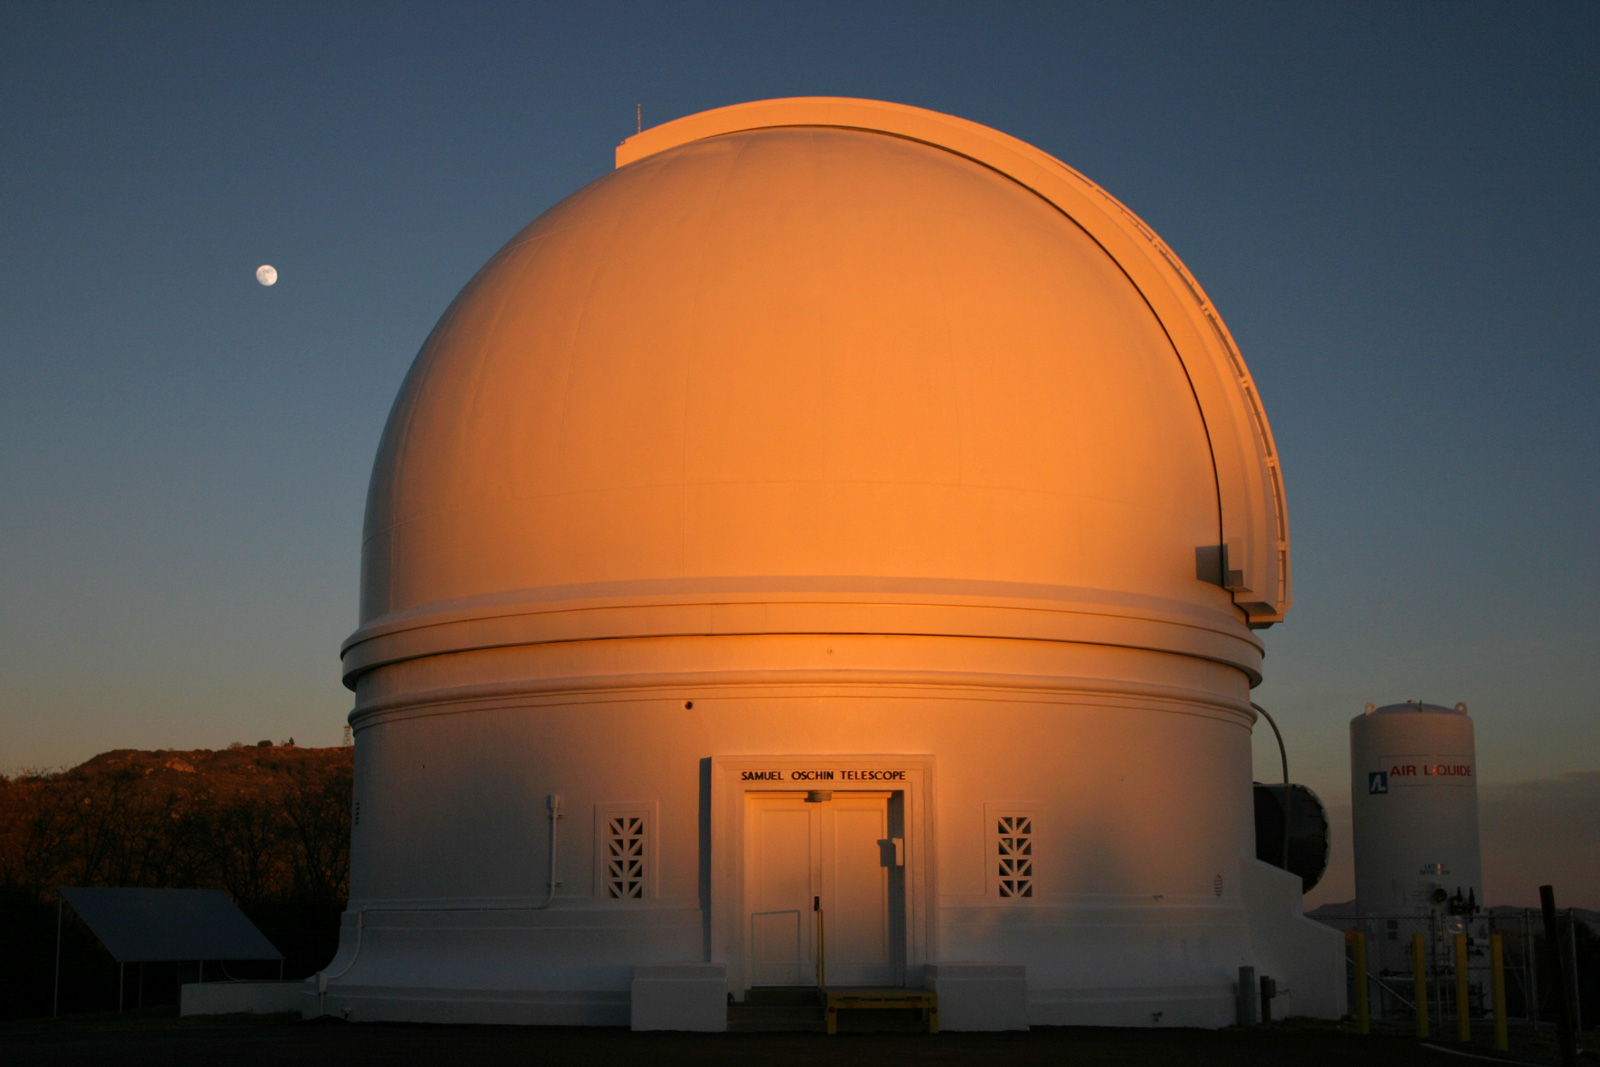
\includegraphics[width=.9\textwidth]{figures/ZTF_dome.jpg}
		\caption{Telescope P48 utilisé par ZTF \\ \credits{Caltech/Palomar}}
	\end{figure}
\end{column}
\end{columns}

\end{frame}

\subsection{DESI}

\begin{frame}{Uchuu BGS}
\begin{columns}
\begin{column}{.5\textwidth}
	\begin{itemize}
		\item Utilise le Mayall Telescope à l'Observatoire de Kitt peak 
		\item 4m de diamètre pour un champ de 8.0 degrés carré
		\item 5 000 fibres robotisées
		\item  
	\end{itemize}
\end{column}

\begin{column}{.5\textwidth}
	\begin{figure}
		\centering
		\includegraphics[width=0.9\textwidth]{figures/Artistic_DESI.jpg}
		\caption{Vue d'artiste du Mayall Telescope et des données DESI Y1 \\ \credits{DESI Collaboration/KPNO/NOIRLab/NSF/AURA/P. Horálek/R. Proctor}}
	\end{figure}
\end{column}

\end{columns}
\end{frame}

\subsection{Observations}

\begin{frame}{Observations}
\begin{figure}
	\centering
	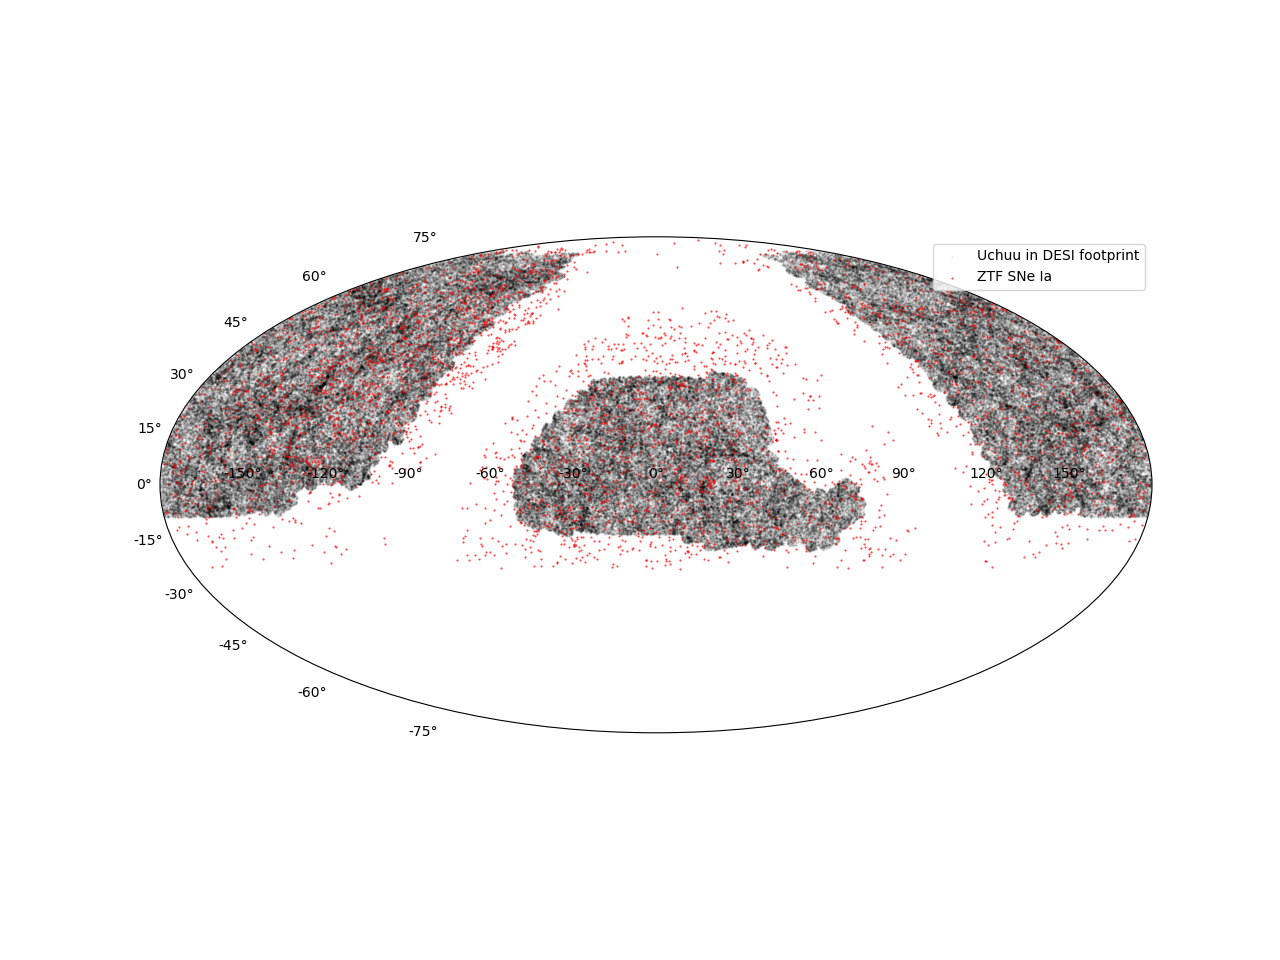
\includegraphics[width=0.9\textwidth, trim = {3cm, 5cm, 2cm, 5cm}, clip]{figures/ZTF_on_DESI.png}
	\caption{Événements réels observés par ZTF et footprint DESI}
\end{figure}
\end{frame}

\begin{frame}{Contexte}
\begin{figure}
	\centering
	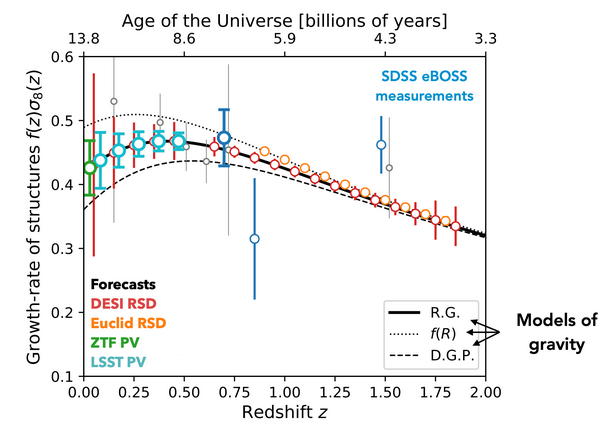
\includegraphics[height=0.7\textheight]{figures/fs8.png}
	\caption{Gain apporté par les vitesses particulières des SNe sur $f\sigma_8$}
\end{figure}
\end{frame}

\begin{frame}{Objectifs du stage}
\begin{enumerate}
\item Générer des supernovae incluant des effets de vitesses particulières
\item Permettre un test du pipeline \lemaitre
\item vp pour fs8
\end{enumerate}
\end{frame}

\section{Chaîne d'analyse cosmologique avec SNe Ia}


% Suivre la reconstruction d'une SNe

\subsection{Générations des SNe}

\begin{frame}{Générations des SNe}
Skysurvey
position selon Uchuu
\begin{figure}
	\centering
	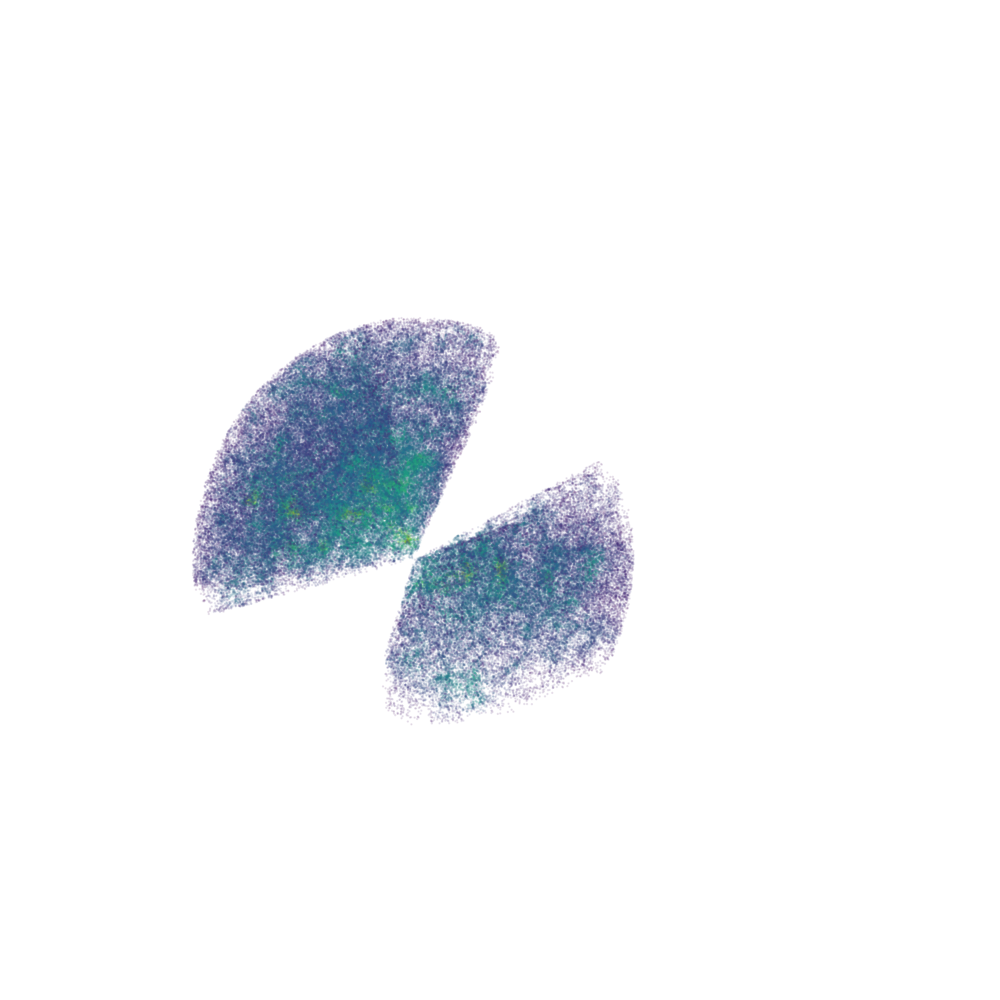
\includegraphics[height=2cm, trim={2cm 2cm 2cm 2cm}, clip]{figures/Uchuu.png}
	\caption{Simulation Uchuu}
\end{figure}
paramètres x0 x1 c tmax
\end{frame}

\begin{frame}{Courbes de lumière et spectres}
	pictures
\end{frame}

\subsection{Reconstruction des paramètres de standardisations}

\begin{frame}{Paramètres de standardisations}
Salt/NaCl
\end{frame}

\subsection{Reconstruction des distances et de la cosmologie}

\begin{frame}{Reconstruction des distances et de la cosmologie}
EDRIS
\end{frame}

\subsection{Reconstruction des vitesses particulières}

% Préciser que c'est grâce à ZTF qu'on peut avoir des vp, car bas redshift et précision

\begin{frame}{Vitesses particulières}
Interpolation pour $z(\mu)$, puis $v_{pec} = c(z_{obs} - z(\mu))$
\end{frame}

\section{Résultats}

\subsection[Contribution dans \textsc{Lemaître}]{Exemple de contribution dans la chaîne~: Réglages de hyperparamètres dans NaCl}

\begin{frame}{Réglages de hyperparamètres dans NaCl}
Contraintes et régularisations
 
\end{frame}

\subsection{Vitesses particulières obtenues}

\begin{frame}{NaCl vs Salt2.4}

\end{frame}

% Potentiellement effet extinction galactique si implémentée d'ici-là

\section{Conclusion}

\begin{frame}{Conclusion}

\end{frame}

\begin{frame}{Persepectives}

\end{frame}





\end{document}